\chapter{Magnetické vázání}

Velmi důležitým jevem, který jsme při dalším experimentování objevili, je, že dva spinnery umístěné blízko sebe, z nichž jeden je poháněn motorem\footnote{Tento spinner nazveme hnacím.}, se mohou magneticky vázat - tzn. že si hnaný a hnací spinner udržují nějaký konstantní poměr rychlostí.
Tomu, v jakém poměru jsou, budeme říkat "mód"; případ, kdy jsou rychlosti hnaného a hnacího spinneru stejné bude, tedy mód 1 ku 1 (značeno 1:1). Později v této kapitole budeme tyto módy dále zkoumat a budeme vždy prvním číslem označovat rychlost hnaného spinneru a druhým číslem rychlost hnacího spinneru. Tento jev je obvzlášť důležitý, jelikož umožňuje tvorbu prvního primitivního druhu magnetického převodu.

\section{Měření magnetickým čidlem}

\clearpage
\section{Vylepšení aparatury}

\subsection{Laserový snímač}

\begin{wrapfigure}{r}{0.45\textwidth}
    \vspace*{-0.75cm}
    \includegraphics[width=0.30\textwidth]{laser_tracking_circle16.png}
    \centering
    \caption[Obrázek použitého absorpčního kola]{Obrázek použitého absorpčního kola (16 výsečí) na našich spinnerech. Vyšší počet výsečí je možný, ale 16 bylo pro náš případ dostačující. Šedivá výseč tvoří referenční bod, podle kterého je možné v kódu určit přesnou rotaci vůči okolí. }
    \label{fig:laser_circle16}
\end{wrapfigure}

Dříve použité metody snímání pohybu spinnerů mají své výhody i nevýhody. Nevýhodou snímání pomocí magnetickéh čidla je nízká přesnost a nevýhodou snímání pomocí videa je pracnost následného trackování a časová limitace záznamu. 

Dalším krokem k vylepšení naší aparatury tedy bylo vytvořit lepší způsob snímání. K tomuto jsme se rozhodli vytvořit vlastní senzory postavené na snímání absorpce laserového paprsku fotodiodou. Na každý spinner pak byl připevněn papírový disk  se střídajícími se černými a bílými pruhy (viz \autoref{fig:laser_circle16}), které jinak absorbují světlo z laseru, čímž se mění i měřené napětí na fotodiodě. Z průběhu napětí měřeného osciloskopem jsme podobně jako v kódu \ref{code:4} schopni určit úhlovou rychlost.

\begin{wrapfigure}{r}{0.45\textwidth}
    \includegraphics[width=0.45\textwidth]{laser_setup_0.png}
    \centering
    \caption{Ilustrace použití laserového snímače (LS)}
    \label{fig:laser_circle16}
\end{wrapfigure}
Nyní jsou našimi limitacemi pouze: vzorkovací frekvence osciloskopu, která je pro naše využití více než dostačující, a počet pruhů na papírovém kole, který můžeme dle libosti měnit.

\subsection{Zbytek aparatury}

Celá aparatura využívá 2 laserové snímače - jeden pro hnací spinner a jeden pro hnaný spinner. Hnací spinner je poháněn motorem, resp. vrtačkou, jejíž otáčky jsou regulovány laboratorním zdrojem napětí. Hnaný spinner je poté pevně upevněn v definované vzdálenosti od hnacího.
\clearpage

